%
%  Vincent Yannello
%
\documentclass[12pt,fullpage]{article}
\usepackage{fullpage}
\usepackage{amsmath}
\DeclareMathOperator{\erf}{erf}
\usepackage{psfrag}                                          % LaTeX graphics tool
\usepackage{pslatex}                                         % avoids the default cmr font
\usepackage{graphicx}                                        % graphics package 
\usepackage{epsfig}                                          % figures
\usepackage{hyperref}
\usepackage{color}

\begin{document}

\noindent
{\bf Logarithm distribution} (from \color{blue}\url{http://www.math.wm.edu/~leemis/chart/UDR/UDR.html}\color{black})

\noindent
The shorthand $X \sim {\rm logarithm}(c)$ is used to indicate that the
random variable $X$ has the logarithm distribution with parameter $c$.
A logarithm random variable $X$ with parameter $c$ has probability mass function 
$$
f(x) = -{\frac { \left( 1 - c \right) ^ {x}} {x \ln  \kern -0.08 em c }
} \qquad \qquad x = 1, 2, \ldots
$$
for any $0 < c < 1$.
The probability mass functions for two different values of $c$ are illustrated below.
\begin{figure}[h!]
\begin{center}
\psfrag{labf}{$f(x)$}
\psfrag{labx}{$x$}
\psfrag{labp1}{$c = 0.1$}
\psfrag{labp2}{$c = 0.5$}
\includegraphics[width=5.6in]{LogarithmPlot.ps}
\end{center}
\end{figure}\\
The cumulative distribution, survivor function, hazard function, cumulative hazard 
function, and inverse distribution function on the support of $X$ are mathematically intractable.
\\
\\
The moment generating function of $X$ is
$$
M(t) = E \left[ e ^ {\kern 0.08 em tX} \right] = \frac {\ln  \kern -0.08 em \left( 1 - {e ^ {\kern 0.08 em t}} + {e ^ {\kern 0.08 em t}} c \right) }{\ln  c } \qquad \qquad -\infty < t < \infty.
$$
The characteristic function of $X$ is
$$
\phi(t) = \frac {\ln  \left( 1 - {e ^ {\kern 0.08 em it}} + {e ^ {\kern 0.08 em it}}c \right) }{\ln  \kern -0.08 em c
 } \qquad \qquad -\infty < t < \infty.
$$
The population mean and variance of $X$ are
$$
E[X] = {\frac {c - 1}{c \ln  c}} \qquad \qquad 
V[X] = {\frac { \left( c - 1 \right)  \left(\ln  \kern -0.08 em \left( c \right)+ 1 - c
 \right) }{ \left( \ln \kern -0.08 em c \right) ^ {2}{c} ^ {\kern 0.04 em 2}}} \qquad \qquad 
$$
The skewness and kurtosis can be determined using the APPL code below.
\vspace{0.1in}

\newpage
\noindent
{\bf APPL verification:}
The APPL statements
\begin{verbatim}
assume(0 < c < 1);
X := [[x -> -(1 - c) ^ x / (x * log(c))],[1 .. infinity], ["Discrete", "PDF"]];
Mean(X);
Variance(X);
Skewness(X);
Kurtosis(X);
MGF(X);
\end{verbatim}
verify the population mean, variance, skewness, kurtosis, and moment generating function.

\end{document}
